\section{The Models Language and Architecture}

Metadata Registries are needed in organizations to ensure data consistency. Metadata Registries are capable of analysing, administering and classifying metadata and very often in practise they also function as repositories for metadata, storing the schema and blueprints for data types and structures. The ideas and concepts that are stored in data systems form the basis of executable software systems, however many of the details are peculiar to particular disciplines.  

In the past Data Dictionaries were used to store details of database record structure or application data structure on a local per application basis, a metadata registry provides a similar capability but on a system or organisation-wide basis. It also provides features that are commonly included in a \emph{thesaurus}, a \emph{Taxonomy}, and an \emph{Ontology} . These features include the ability to classify terms in relation to one another, record relationships such as synonyms, and classify hierarchical relationships.

Metadata Registries are normally found in Data Warehouses and Enterprise systems, where vast quantities of data need to be administered and managed. It is likely that metadata registries will become more common as it becomes more and more necessary to deal with the recent internet-driven data explosion, especially as much of this data is unstructured, and can only be processed by relatively inefficient techniques.

Metadata Registries contain the ability to examine both how a data element is represented as well as what it means, and it is this relationship that is embodied in the International Standard 11179, which I will examine in the next section. There are other standards which purport to be concerned with metadata registries namely ISO15000-3 and ISO15000-4, which relate to ebXML, however they are more concerned with storing and accessing metadata rather than classifying it and relating the semantic and representational aspects of that metadata.

This chapter takes key concepts from the ISO11179 standard and explores ways in which these concepts can be integrated with concepts and ideas embodied in the Meta-Object Facility (MOF) model-driven engineering standards in order to design a metadata registry, which will both serve the practical purpose of allowing datasets to be matched, compared and managed, and allow for the development of a unified treatment of data in heterogeneous systems. The first part looks at the ISO standard and the ideas behind MOF, the second takes these ideas and uses them as the foundation for a specification of a metadata registry. The third section looks at how the metadata registry can be used to provide basic services for data-oriented model driven programming. In later chapters the practical and theoretical problems are examined in detailed to see in what ways full automated semantic interoperability can be achieved.


\section{Metadata Registries - An Overview of Standards and Ideas}
\subsection{ISO11179}
ISO11179 is the international standard relating to metadata and in particular metadata registries, and although there are a few other related standards which I have examined in the course of specifying a metadata registry ISO11179 provides the most exhaustive description of a metadata registry. It is therefore a key reference in this specification. If we abstract the core ideas from the ISO11179 standard we have the notion of a \emph{data element concept}, \emph{a data element}, \emph{a value domain}, and a \emph{conceptual domain}. There is a four-way set of relationships between CDs, VDs, CDEs, and DECs which draws a distinctions between the conceptual or semantic \emph{level} and the representational \emph{level} in which these entities live, illustrated in figure\ref{fig:overviewMDR}.


\begin{figure}[here]
	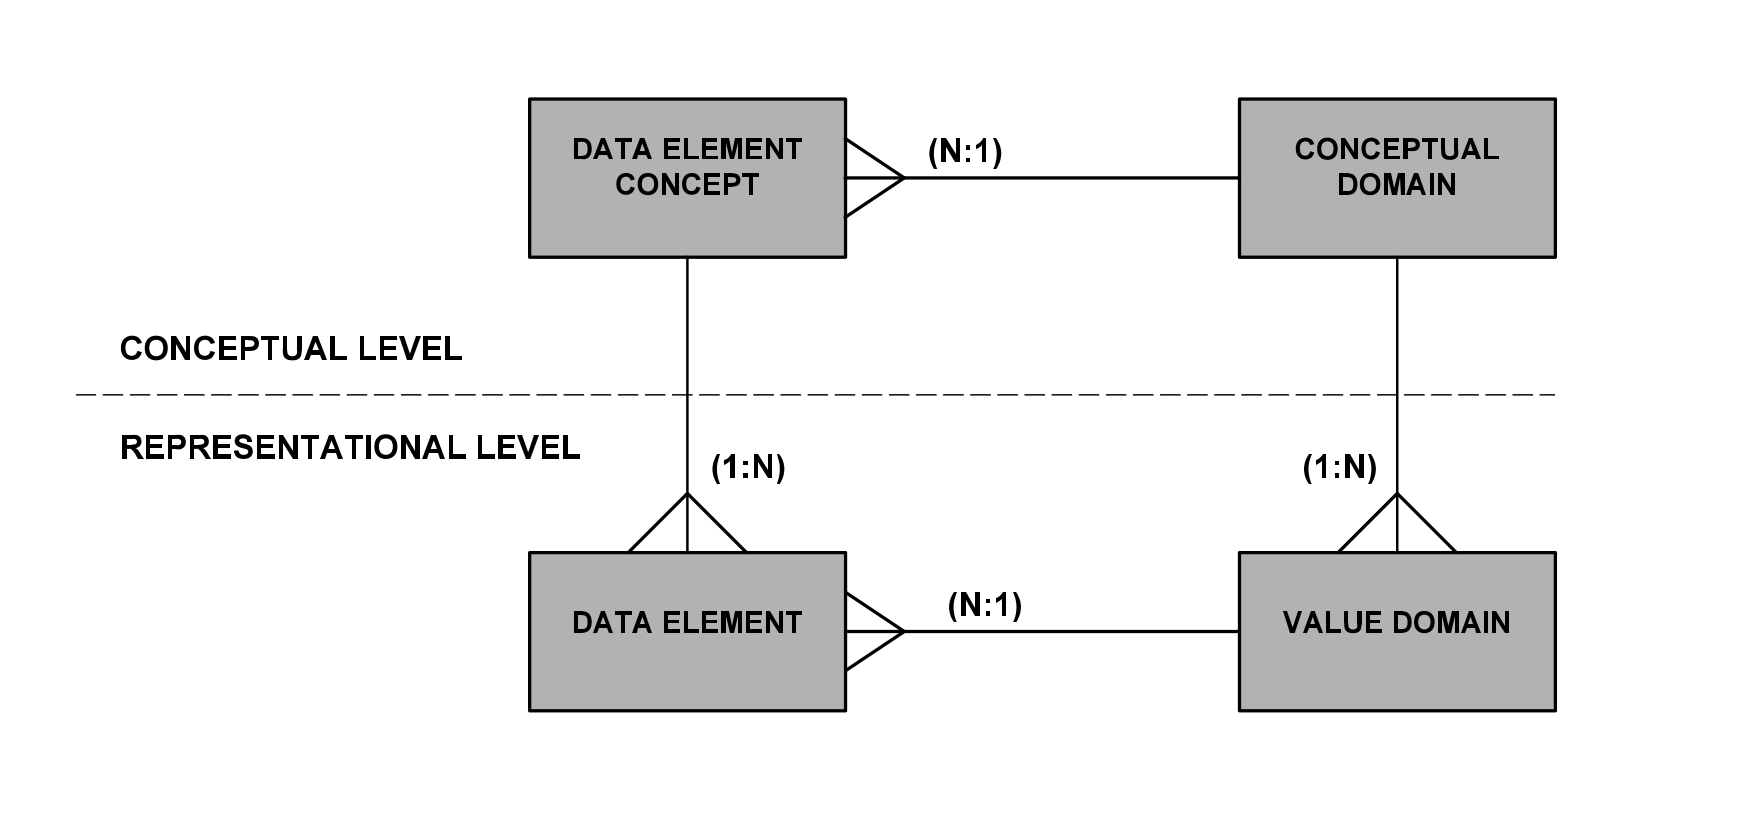
\includegraphics[width=0.5\textwidth,natwidth=610,natheight=642]{Overview11179}
	\caption{Overview model for a Metadata Registry} 
	\label{fig:overviewMDR}
\end{figure}

We can get some more hints as to the theory behind these guidelines in a related ISO standard \emph{ISO 20943-1: the standard relating to achieving consistency in meta-data registries)} which states that the data element concept may relate several data elements that record data about that concept with different representations, implying that a single data element concept may have many value domains. It would appear therefore that what is intended is that a common data element in ISO11179 is really a relationship, or mapping between the set of data element concepts and the set of value domains. Therefore a list of data elements as DEL can be represented as follows:
\vskip 4mm
\begin{axdef}DEL : DEC \rel VD\end{axdef}
\vskip 4mm
The relationship between DEC's and VD's can be viewed as a set of mappings. If we look at the mapping from VD to DEC then this is a mapping rather than a function, every VD must be related at least one DEC, but it could of course be related to more than one.  An Integer data-type in a programming language may be used to represent inches in a measurement program, it may also be used to count tanks in a logistics application. It is also likely that since we are representing concepts in a physical domain, which by definition has many more constraints acting on it there will always be a many DECs for every VD.
A data element is said to be comprised of a data element concept(DEC) which is its meaning and a value domain(VD) which is its representation. But how exactly is this relationship built up? and how can it be replicated? 
If we turn to the ISO standards we obtain these definitions:
\vskip 4mm 

\begin{table}[h]
	\begin{tabular}{ p{1.8cm} p{2.8cm}  p{3.0cm}  }  % centered columns (2 columns)
		\hline
		Entity & ISO Definition & ISO11179 Implementation Guidelines  \\ 
		\hline
		Data Element Concept(DEC) & An idea that can be represented in the form of a data element, described independently of any particular representation. & A concept that can be represented in the form of a Data Element, described independently of any particular representation.\\
		Common Data Element(CDE) & A unit of data for which the definition, identification, representation, and permissible values are specified by means of a set of attributes. & A unit of data for which the definition, identification, representation and Permissible Values are specified by means of a set of attributes. \\
		Value Domain (VD) & The description of a value meaning. & A description of a Value Meaning. \\
		Conceptual Domain (CD) & A set of valid value meanings, which may be enumerated or expressed via a description.& A set of valid Value Meanings.\\
		\hline
	\end{tabular}
\end{table}

\vspace{5.mm}


The simple mapping between DEC's and VD's is perhaps better replaced with a functional relationship, and in section 2 we will explore the idea of a functional relationship between the two, its advantages and disadvantages. For now we will just try and describe the MDR according to the ISO specification. If we consider a single model of a system then we are putting constraints on the extent of the VD's, or if a set of VD's is considered to be a conceptual domain then we are constraining the model to a single CD.  By doing this we can model the system using functional relationships, so make a total function relating the model DEC's to the VD's \emph{in a particular conceptual domain}, since all the DEC's will have a mapping to a VD. It is not an injective function because of course more than one DEC can use the same representation or VD, and it is not surjective because there can be VD's in that particular Conceptual Domain which are not used in the model. It may be that a more useful model can be built by using the term Conceptual Domain to mean just those elements related to a \emph{group} of data elements, in which case we could specify a surjective relationship.  The ISO standard does not specify anything about \emph{groups} of data elements, so it would be perfectly reasonable to introduce just such a constraint. 


As an illustration lets take the case of a marine systems model in which there may be a data element, say depth below sea-level, which is being recorded in the event that the naval vessel on which the instrument is placed is a submarine.  However it may not be, in which case no actual values of depth will be recorded, measured or used in the system. In the implementation therefore we are using the set of value domains mapped to actual values (VAL), and so the actual depth (AD) can be viewed as a partial function:
\vskip 4mm 
\begin{zed}
	[VAL]\\
	AD == VD \pfun VAL
\end{zed}
\vskip 4mm 
since while the vessel is on the surface we have nothing recorded and thus no VD mapping to a VAL, or AD == \{\}.  

Consider the definition of a \emph{Conceptual Domain}:
\begin{quote}
	A conceptual domain is a set of value meanings. The intension of a conceptual domain is its value meanings. Many value domains may be in the extension of the same conceptual domain, but a value domain is associated with one conceptual domain. Conceptual domains may have relationships with other conceptual domains, so it is possible to create a concept system of conceptual domains. Value domains may have relationships with other value domains, which provide the framework to capture the structure of sets of related value domains and their associated concepts.
	
\end{quote}


\subsection{A Metadata Language and Abstract Architecture }

The ISO11179 specification illustrates different aspects of the standard using UML class diagrams, we have used these to inform the development of a very simple domain specific language based on the standard. The main differences are that we have added in containers to handle data element collections, calling these \emph{Models} and to handle collections of these \emph{Models} which we have called \emph{Classifications}.

A simplified overview model, without attributes and methods, is shown in Figure \ref{fig:basicMDR}.

\begin{figure}[here]
	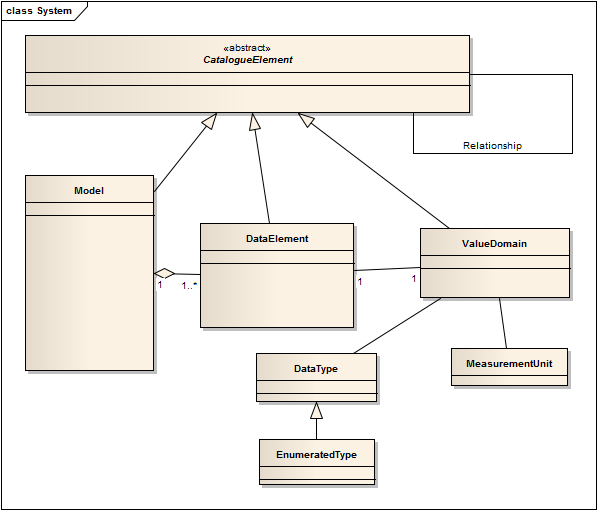
\includegraphics[width=0.5\textwidth,natwidth=610,natheight=642]{MCSimplifiedOverview}
	\caption{Overview model for a Metadata Registry} 
	\label{fig:mcSimplifiedOverview}
\end{figure}



 




